%%%%%%%%%%%%%%%%%%%%%%%%%%%%%%%%%%%%%%%%%%%%%%%%%%%%%%%%%%%%%%%%%
\begin{frame}{Formuling a SIS-SDE}
    \begin{overlayarea}{\textwidth}{\textheight} 
        Now, consider $\{I_t\}_{t \geq 0}$. 
        \only<2->{
            For fixed time $t$
            $I_t$ is a r.v, assume that  $I_t$
            has a probability density 
            function $p(x,t)$.
        }
        \only<3->{
            That is,
            \begin{equation*}
                \probX{a \leq I_t \leq b}
                    = \int_{a}^{b}
                    p(x,t) dx.
            \end{equation*}
        }
        %     
        \only<4->{
            $I_t$ is Markovian.
        }
    %  
        \only<5->{
            \begin{align*}
                &\probCX{I_{t_{n}} \leq y}{I_{t_0}, \cdots, I_{t_{n-1}} }
                    =
                        \probCX{ I_{t_{n}} \leq }{I_{t_{n-1}}}
                    \\
                        \text{for all } &
                        0 \leq t_0 < t_1 < \cdots < t_n
            \end{align*}
        }
        
        \only<6->{
            Denote the transition p.d.f as
            \begin{align*} 
                & p(y, t + \Delta t; x ,t)
                \\
                & y = I_{t + \Delta t},
                \quad x =I_t
        \end{align*}
        }
    \end{overlayarea}
\end{frame}
%%%%%%%%%%%%%%%%%%%%%%%%%%%%%%%%%%%%%%%%%%%%%%%%%%%%%%%%%%%%%%%%%%%%%%%%%%%%
\begin{frame}{}
     Set $\Delta i = 1$, then
    \begin{overlayarea}{\textwidth}{\textheight}
         \begin{align*}
            \only<2->{
                \frac{d p_i}{dt} 
                    =&
                    p_{i -1} b(i-1) + p_{i + 1} d(i + 1)
                    - p_i [ b(i) + d(i)]
            }
            \\
            \only<3->{
                &=
                - \frac{
                    p_{i + 1}[d(i + 1) - d(i + 1)]
                    - 
                    p_{i - 1}[d(i -1) - d(i - 1)]
                }{2 \Delta i}           
            \\
                & +
                \frac{1}{2}
                \frac{
                    p_{i + 1}[d(i + 1) + d(i + 1)]
                    -
                    2 p_i[b(i) + d(i)]
                    +
                    p_{i - 1}[d(i -1) + d(i - 1)]}{
                        (\Delta_i) ^ 2
                    }
            }
        \end{align*}       
        \only<4->{
            Let $i = x$, $\Delta i = \Delta x$ and $pi(t) = p(x,t)$.
            Thus, letting  $\Delta x \to 0$, we obtain the FKE
        }
        \only<5->{
            \begin{align*} 
                \frac{\partial p(x,t)}{\partial t}
                    =&
                        \frac{\partial}{\partial x} \{   
                                [b(x) - d(x)] p(x,t)
                            \}
                    +
                        \frac{1}{2}
                            \frac{\partial ^ 2}{\partial t ^ 2} \{
                                b(x)  + d(x) p(x,t) 
                            \}
                    \\
                    =&
                        \frac{\partial}{\partial x}
                        \left \{
                            \left [
                                \frac{\beta}{N}
                                x (N - x)
                                - (b + \gamma) x
                            \right]
                            p(x,t)
                        \right \}
                    \\    
                    &+
                        \frac{1}{2}
                        \frac{\partial ^ 2}{\partial x ^ 2}
                        \left \{
                            \left [
                                \frac{\beta}{N}
                                    x (N -x) + (\beta + \gamma) x 
                            \right ] p(x, t)
                        \right \}
            \end{align*}
        }
    \end{overlayarea}
 \end{frame}
%%%%%%%%%%%%%%%%%%%%%%%%%%%%%%%%%%%%%%%%%%%%%%%%%%%%%%%%%%%%%%%%%%    
\begin{frame}{}
    Using the SIS-CTMC probablity transition kernel 
    \begin{overlayarea}{\textwidth}{\textheight}
        \begin{align*}
            &p_{ji}(\Delta t):=
                \begin{cases}
                    \frac{\beta i (N - i)}{N} \Delta t 
                        + o(\Delta t),     
                        & j = i + 1
                    \\
                    (b + \gamma) i \Delta t 
                        + o(\Delta t),
                        &   j = i - 1
                    \\
                    1 - \left [
                            \frac{\beta i (N - i)}{N} +
                            (b + \gamma) i %                
                        \right] \Delta t
                        + o(\Delta t) , 
                        & j=i
                    \\
                    o(\Delta t) & \text{otherwise}.
                \end{cases}
        \end{align*}
        \only<2->{
            If increment $\Delta t$ follows a 
            exponential distribution  and is suficiently small.
            Results that increment 
            $$
                \Delta I = I_{t + \Delta t} - I_t
            $$  
            has normal distribuition, with following expectation and variance.
            \\
        }
        \only<3->{
            Fix time $t$ s.t  $I_t = i$
            \begin{align*}
                \E{\Delta I}
                    =&
                        b(I_t) \Delta t - d(I_t) \Delta t + o(\Delta t)
                    \\
                    &=
                        \underbrace{
                            [b(I)_t - d(I_t)]
                        }_{:=\mu(I_t)} + o(\Delta t) 
            \end{align*}
        }
    \end{overlayarea}
\end{frame}    
%%%%%%%%%%%%%%%%%%%%%%%%%%%%%%%%%%%%%%%%%%%%%%%%%%%%%%%%%%%%%%%%%%%%%%%%%%%%
\begin{frame}{}
    Thus
    \begin{overlayarea}{\textwidth}{\textheight}
        \only<2->{
            \begin{align*}
                \VarX{\Delta I_t}
                    &=
                        \EX{\Delta I_t ^ 2} - [\EX{\Delta I_t}] ^ 2
                    \\
                    & = 
                        \underbrace{
                            [b(I_t)  + d(I_t) ]
                        }_{:=\sigma^2(I_t)}
                            \Delta t + o(\Delta t).
            \end{align*} 
        }
        \only<3->{
            Since 
            $
                \Delta I_t \sim \mathcal{N}
                    (
                    \mu(I_t) \Delta t, 
                    \sigma ^ 2 (I_t) \Delta t
                )
            $,
            we see that 
        }
        \only<4->{
            \begin{align*}
                I_{t+\Delta t} 
                    &= 
                        I_t + \Delta I_t
                \\
                    &\approx
                        I_t + \mu(I_t)\Delta t 
                        + \sigma(I_t) \sqrt{\Delta t} \eta
                \\
                    & \eta \sim \mathcal{N}(0,1)
            \end{align*}
            The Euler-Maruyama's recurrence equation.
        }
    \end{overlayarea}
\end{frame}
%%%%%%%%%%%%%%%%%%%%%%%%%%%%%%%%%%%%%%%%%%%%%%%%%
\begin{frame}{}
    \begin{overlayarea}{\textwidth}{.8\textheight}
        Further, becouse under this setting, the Euler-Maruyama converge.   
        \only<2->{
            Letting $\Delta t \to 0$, we deduce our SIS-SDE:
            \begin{equation*}
                dI_t = \mu(I_t) + \sigma(I_t) dW_t.
            \end{equation*}
        }
        \only<3->{
            Sustituting, the notation for birth and death processes
            \begin{equation*}
                dI_t =
                    \frac{\beta}{N} I_t(N - I_t)
                    - (b + \gamma) I_t
                    +
                    \sqrt{
                        \frac{\beta}{N} 
                            I_t (N - I_t)
                            +
                            (b + \gamma)I_t
                    }
                    dW_t.
            \end{equation*}
        }
    \end{overlayarea}
\end{frame}
%%%%%%%%%%%%%%%%%%%%%%%%%%%%%%%%%%%%%%%%%%%%%%%%%%%%%%%
\begin{frame}{}  
    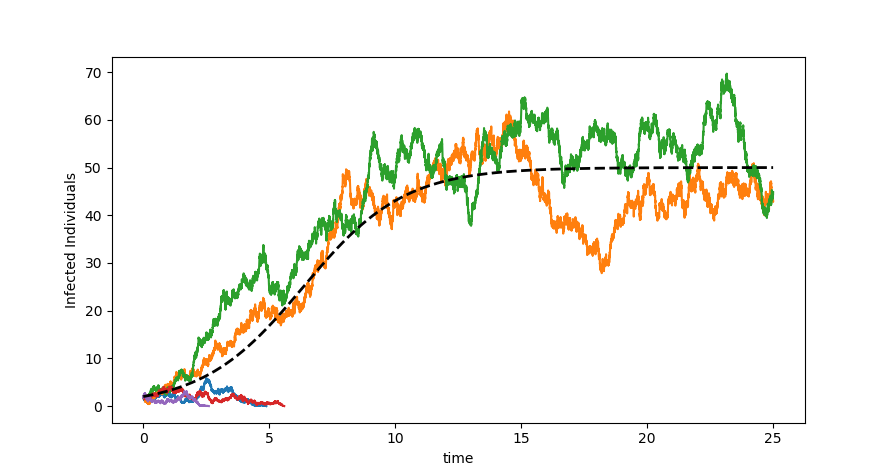
\includegraphics[width=\textwidth,keepaspectratio=true]{%
        noise/Images/Assets/random_walk_SIS-SDE.png%
    }
\end{frame}
